\chapter{Biolog\'ia}
\label{biologia}
\epigraph{Essentially, all models are wrong, but some are useful.}%
{George E. P. Box}

Siendo este un trabajo desde la Ciencia de la Computaci\'on, ser\'ia absurdo
intentar abordar rigurosamente todos los conceptos biol\'ogicos involucrados
en, por ejemplo, la replicaci\'on de un virus dentro de una c\'elula. Al mismo
tiempo, para poder comprender la complejidad del problema que este trabajo se
propone resolver y las decisiones que se tomaron a la hora de implementar el
software, es necesario contar con ciertas definiciones y conceptos biol\'ogicos
elementales que veremos a continuaci\'on.

\section{Lo esencial}
\label{bio-esencial}

M\'as all\'a de la complejidad que existe dentro de un c\'elula, sus componentes
y funcionamiento, se destacan tres macro mol\'eculas fundamentales compuestas
por mol\'eculas peque\~nas:
\begin{itemize}
 \item \ac{DNA} y \ac{RNA} - compuestas por nucle\'otidos. 
 \item Prote\'ina - compuesta por amino\'acidos.
\end{itemize}

\subsubsection{El dogma central}

El dogma central de la biolog\'ia molecular establece que la informaci\'on
fluye del \ac{DNA} al \ac{RNA} y luego a las prote\'inas.
\begin{center}
 \textbf{DNA} $\longrightarrow$ \textbf{RNA} $\longrightarrow$
\textbf{Prote\'inas}
\end{center}

Por supuesto, \'este es un modelo extremadamente simplificado al que le faltan
componentes fundamentales para que todo funcione como corresponde. Podemos
empezar diciendo que las flechas del modelo, implican transformaciones
moleculares y, por lo tanto, existen entidades encargadas de llevar adelante
estas transformaciones. 

La entidad que transforma el \ac{DNA} en \ac{RNA} se denomina \ac{RNA}
polimerasa, y el proceso de transformaci\'on se conoce como
\textit{transcripci\'on}. Por otro lado, la entidad que transforma el
\ac{RNA} en prote\'inas se denomina ribosoma, y el proceso de esta
transformaci\'on es conocido como \textit{traducci\'on}.

\subsubsection{\'Acidos nucleicos}

Ambos \ac{DNA} y \ac{RNA} son, como mencionamos anteriormente, macro mol\'eculas
compuestas por mol\'eculas peque\~nas. Estas mol\'eculas peque\~nas que los
componen se denominan nucle\'otidos. Para definir en detalle a los
nucle\'otidos, deber\'iamos profundizar en conceptos qu\'imicos que no son
relevantes para este trabajo. Sin embargo, podemos decir que en el \ac{DNA}
aparecen 4 nucle\'otidos, \ac{A}, \ac{G}, \ac{T} y \ac{C}, mientras que en el
\ac{RNA} la \ac{T} es reemplazada por \ac{U}. Estos nombres, se corresponden
con la base nitrogenada que conforma cada nucle\'otido y que es lo que
diferencia uno del otro. Luego, tanto el \ac{DNA} como el \ac{RNA} suelen
describirse por su secuencia de nucle\'otidos.

El \ac{DNA} se presenta como una doble cadena de nucle\'otidos, en la que las
dos hebras est\'an unidas a trav\'es de las bases complementarias (reglas de
Watson-Crick\footnote{Fracis H. Crick y James D. Watson recibieron en 1962 el
Premio Nobel en Fisiolog\'ia o Medicina.}), \ac{A} con \ac{T} y \ac{C} con
\ac{G}.

En contraste con el \ac{DNA}, el \ac{RNA} se presenta como una cadena simple de
nucle\'otidos. No obstante esto, el \ac{RNA} tambi\'en puede plegarse siguiendo
las reglas de Watson-Crick (\ac{A}-\ac{U}, \ac{C}-\ac{G}) e inclusive usando
pares menos estables como \ac{A}-\ac{G}. Esto da lugar a lo que se conoce
como la estructura secundaria y que veremos con mayor detenimiento m\'as
adelante.

El concepto de ``estabilidad'' que se acaba de mencionar esta relacionado con
la cantidad de energ\'ia libre que se genera como consecuencia de la uni\'on de
dos bases de nucle\'otidos. Generalmente, predominan las uniones entre bases con
menor energ\'ia libre (m\'as estables), aunque \'esto no siempre es as\'i.

\subsubsection{Prote\'inas}

Al igual que lo \'acidos nucleicos, las prote\'inas son macro mol\'eculas
compuestas por mol\'eculas peque\~nas, pero en este caso las mol\'eculas que
las componen, se denominan amino\'acidos. Tambi\'en al igual que con los
nucle\'otidos, dejaremos de lado la descripci\'on qu\'imica de los
amino\'acidos y nos centraremos en los aspectos que son m\'as relevantes para
este trabajo.

Existen 20 amino\'acidos diferentes que suelen representarse por su nombre
abreviado (usando tres letras o una letra). Las prote\'inas son esencialmente
secuencias de al menos 50 amino\'acidos y son responsables de diferentes tareas
fundamentales para el correcto funcionamiento de la c\'elula. Sin ir mas lejos,
el proceso de traducci\'on, es decir, la s\'intesis de prote\'inas, lo realizan
los ribosomas, que est\'an compuestos en parte por prote\'inas\footnote{El
lector se preguntar\'a ?`qu\'e fue primero, el ribosoma o la prote\'ina?.}.

\subsubsection{Del \ac{DNA} a las prote\'inas}

Como ya vimos m\'as arriba, el dogma central nos dice que la informaci\'on en la
c\'elula fluye desde el \ac{DNA} hasta convertirse en prote\'inas a trav\'es de
transformaciones moleculares denominadas \textit{transcripci\'on} y
\textit{traducci\'on}. Tambi\'en vimos, muy brevemente, que tanto el \ac{DNA}
como el \ac{RNA} est\'an compuestos por nucle\'otidos mientras que las
prote\'inas est\'an compuestas por amino\'acidos. No profundizaremos en los
procesos de transcripci\'on y traducci\'on, pero s\'i nos interesa ver como se
traducen los nucle\'otidos a los amino\'acidos.

Para esto necesitamos introducir el concepto de c\'odigo gen\'etico. El
c\'odigo gen\'etico es, precisamente, el conjunto de normas o reglas con las
cuales el material gen\'etico (secuencia de nucle\'otidos) se traduce en
prote\'inas (secuencia de amino\'acidos). El c\'odigo define una relaci\'on
entre secuencias de 3 nucle\'otidos, llamadas codones, y los amino\'acidos. A
cada codon le corresponde a lo sumo un amino\'acido, pero como veremos en
seguida, cada amino\'acido puede estar relacionado con m\'as de un codon.

Como vimos anteriormente, en el \ac{RNA} aparecen 4 nucle\'otidos. Luego,
la cantidad de codones posibles, est\'a dada por $4^{3} = 64$ codones
posibles. Por otro lado, dijimos que existen 20 amino\'acidos, lo que
r\'apidamente nos hace notar que la relaci\'on definida por el c\'odigo
gen\'etico, no puede ser inyectiva. En criollo, la misma secuencia de
amino\'acidos puede ser codificada por distintas secuencias de
nucle\'otidos.

La tabla de c\'odigo gen\'etico indica qu\'e codones se traducen en qu\'e
amino\'acido. Hay amino\'acidos que son representados por tan s\'olo un codon,
mientras otros, son representados hasta por 6 codones. M\'as adelante, veremos
que una de las estrategias para racionalizar el dise\~no de vacunas atenuadas,
se basa en determinar qu\'e codones es conveniente usar para codificar una
secuencia de amino\'acidos determinada, y c\'omo esto afecta la atenuaci\'on del
virus.

Adem\'as, debemos mencionar la existencia de cuatro codones especiales. Estos
codones, uno denominado de \textit{START} y los otros tres denominados de
\textit{STOP}, sirven como indicadores para el proceso de transformaci\'on desde
el \ac{RNA} hasta las prote\'inas (traducci\'on).

Esto \'ultimo es fundamental para delimitar 2 tipos de regiones sobre una
secuencia de \ac{RNA}:
\begin{itemize}
 \item Regiones traducidas: se las denomina \ac{ORF} y son las partes de la
secuencia que efectivamente se traducen en prote\'inas. Puede haber uno o varios
\ac{ORF}, pero cada uno debe empezar con un codon de \textit{START} y terminar
con uno de \textit{STOP}.
 \item Regiones no traducidas: Se las denomina \ac{UTR} y se encuentran a
izquierda y derecha de un \ac{ORF}. Se suele hablar de un 5'-\ac{UTR} y un
3'-\ac{UTR}, para hacer referencia al extremo izquierdo y derecho
respectivamente\footnote{La notaci\'on de 5' y 3' viene de la notaci\'on
utilizada en qu\'imica para numerar los carbonos de un compuesto org\'anico.}.
\end{itemize}

Por \'ultimo, haremos referencia al \ac{IRES}. Un \ac{IRES} es una secuencia de
nucle\'otidos que permite el inicio del proceso de traducci\'on y suele
encontrarse en el 5'-\ac{UTR} de los virus \ac{RNA}. Esta secuencia y la
estructura secundaria que formen, determina en gran medida la s\'intesis de
prote\'inas del virus.

\section{La estructura secundaria de \ac{RNA}}
\label{estructura}
Como ya mencionamos, el plegamiento de una secuencia de \ac{RNA} entre sus bases
complementarias, determina lo que se denomina \textit{estructura secundaria de
\ac{RNA}}. Conocer la estructura secundaria es fundamental para comprender el
funcionamiento de los distintos tipos de \ac{RNA} y de la c\'elula en general.
Existen diferentes tipos de \ac{RNA} pero se distinguen 3 tipos principales: 
\begin{itemize}
 \item \ac{mRNA}.
 \item \ac{rRNA}.
 \item \ac{tRNA}. 
\end{itemize}

Cada uno de estos tipos de \ac{RNA} desarrolla diferentes funciones en el
modelo del dogma central con el fin de lograr las transformaciones moleculares
de transcripci\'on y traducci\'on. Por lo tanto, los plegamientos o estructuras
secundarias que forman determinan en gran medida la actividad celular.

La existencia del t\'ermino \textit{estructura secundaria} nos hace suponer que
existe tambi\'en una \textit{estructura primaria}. De hecho, ya vimos la
estructura primaria de \ac{RNA} cuando dijimos que el \ac{RNA} se suele
representar como una secuencia de nucle\'otidos. Efectivamente, a esta secuencia
se la denomina estructura primaria. Tambi\'en existe la estructura terciaria de
\ac{RNA}, pero la dejaremos de lado por no ser relevante en este trabajo.

\begin{definition}
\label{rna_primary}
Una estructura primaria de \ac{RNA} S, es una secuencia de \ac{RNA} de longitud
$n$, $A=a_{1}a_{2}a_{3}\dots a_{n}$ con $a_{i} \in \left\lbrace A, U, G, C
\right\rbrace$ 
\end{definition}

\begin{definition}
\label{rna_secondary}
Dada una estructura primaria o secuencia de \ac{RNA} de longitud $n$, la
estructura secundaria es un conjunto S de pares $(i,j)$ con $1\leq i < j \leq
n$ tal que para todo, $(i,j), (i',j') \in S$ se satisfacen las tres siguientes
condiciones:
\begin{itemize}
 \item $j-i > 3$
 \item $i=i' \Leftrightarrow j=j'$
 \item $i< i'\Rightarrow i < i' < j' < j \lor i < j < i' < j'$ 
\end{itemize}
\end{definition}

N\'otese que cada base de la secuencia puede estar a lo sumo ``apareada'' o
``unida'' con una sola base, o eventualmente con ninguna. Adem\'as, esta
definici\'on supone la ausencia de \textit{pseudo-knots}. Un
\textit{pseudo-knot} est\'a formado por 2 pares de bases superpuestos, es decir,
$(i,j)$ y $(i',j')$ con $i < i' < j < j'$. Esta suposici\'on se debe
principalmente a que de otra manera, los algoritmos que veremos mas adelante
para la predicci\'on de estructura secundaria, pasan de tener complejidad
polinomial a ser NP-completos\cite{Lyngso00}. Sin embargo, esta suposici\'on
est\'a justificada porque la ocurrencia de \textit{pseudo-knots} es poco
frecuente  en la naturaleza y porque adem\'as pueden ser considerados en
an\'alisis posteriores\cite{Zuker84}.

\begin{figure}
 \centering
  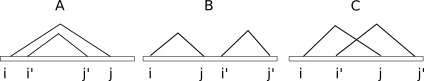
\includegraphics[scale=0.8]{possiblestr}
  \caption{A: $i < i' < j' < j$ B: $i < j < i' < j'$ C: $i < i' < j < j'$}
  \label{possiblestr}
\end{figure}

En la Figura~\ref{possiblestr} se pueden ver las posibles situaciones que se
pueden dar para dos pares $(i,j),(i',j')$ con $i < i'$. Seg\'un la definici\'on
que dimos m\'as arriba, las situaciones en $A$ y $B$ est\'an permitidas mientras
que la situaci\'on en $C$ representa un \textit{pseudo-knot} y estos no son
tenidos en cuenta.

\subsubsection{La estructura secundaria, el \ac{IRES} y la atenuaci\'on de un
virus}

La importancia de la estructura secundaria en este trabajo radica,
fundamentalmente, en su participaci\'on en la s\'intesis de prote\'inas del
virus y en consecuencia, en su atenuaci\'on. Para diferentes virus \ac{RNA}, se
puede decir que la estructura secundaria del \ac{IRES} determina la ``afinidad''
o ``atracci\'on'' con los ribosomas. Luego, esto incide fuertemente en el
proceso de traducci\'on de las prote\'inas que causan la enfermedad, o que
est\'an involucradas en el proceso de replicaci\'on del virus. Una estructura
secundaria con menor afinidad (que la estructura secundaria del virus), le
permitir\'ia al sistema inmune generar los anticuerpos necesarios para
protegerse del virus antes de que se produzca la enfermedad.

\section{Los virus \ac{RNA}}
\label{virus}
Un virus \ac{RNA} es, esencialmente, aquel que tiene el \ac{RNA} como su
material gen\'etico. Adem\'as, los virus suelen clasificarse seg\'un la
``Clasificaci\'on de Baltimore'' que los agrupa en diferentes clases (clase I a
clase VII) seg\'un el tipo de genoma. En particular, en este trabajo se
contemplan los virus \ac{RNA} clase IV tambi\'en llamados \ac{(+)ssRNA virus}

Como ya se mencion\'o en la secci\'on~\ref{motivacion}, una de las
caracter\'isticas de este tipo de virus es su alta frecuencia de mutaciones.
Esto se debe, principalmente, a la alta tasa de error en su \ac{RNA}
polimerasa\footnote{A diferencia de la \ac{DNA} polimerasa que posee la
capacidad de detectar y corregir errores.} (involucrada en el proceso de
replicaci\'on del virus), estimada entre $1\times10^{-3}$ a $1\times10^{-5}$
errores por nucle\'otido por ciclo de replicaci\'on\cite{Vignuzzi08}. Debido a
que los virus de \ac{RNA} suelen tener menos de 10,000 nucle\'otidos, esto se
traduce en 0.1 a 10 mutaciones por genoma replicado.

Si retomamos lo dicho en la secci\'on~\ref{estructura} sobre la ``afinidad''
entre la estructura secundaria y los ribosomas, y c\'omo esto impacta en la
atenuaci\'on del virus, se puede ver que esta alta frecuencia de mutaciones,
conduce a la posibilidad de que en sucesivas replicaciones, el virus sufra
mutaciones que le devuelvan su estructura secundaria original (o similar) y en
consecuencia, pierda su atenuaci\'on.

\subsubsection{Poliovirus}

El poliovirus es un \ac{(+)ssRNA virus} de aproximadamente 7,500 nucle\'otidos
de longitud, miembro del g\'enero \textit{Enterovirus} de la familia
\textit{Picornaviridae} y causante de la poliomielitis. El poliovirus puede
atacar el sistema nervioso y destruir las c\'elulas nerviosas encargadas del
control de los m\'usculos. Como consecuencia, los m\'usculos afectados dejan de
cumplir su funci\'on y se puede llegar a una par\'alisis irreversible. En casos
severos, la enfermedad puede conducir a la muerte.

\subsubsection{La vacuna \ac{OPV}}

Ya presentamos en la secci\'on~\ref{motivacion} la vacuna \ac{OPV} contra la
poliomielitis y sus principales complicaciones. Con los conceptos vistos
hasta el momento, estamos en condiciones de profundizar sobre el por qu\'e de
estas complicaciones.

Se han identificado tres serotipos\footnote{A los fines pr\'acticos y relevantes
en este trabajo, formas en que se presenta un determinado virus.} de poliovirus:
\ac{PV1}, \ac{PV2} y \ac{PV3}. Los tres serotipos son extremadamente virulentos
y producen los mismos s\'intomas de la enfermedad. Para cada uno de estos
serotipos, se desarroll\'o  su correspondiente virus atenuado Sabin 1, Sabin 2 y
Sabin 3 respectivamente, que luego fueron combinados en la vacuna \ac{OPV}.

Cada uno de estos virus atenuados presenta diferentes niveles de riesgo o
probabilidad de revertir a la virulencia. El 90\% de los casos registrados de
\ac{VAPP} son causados por Sabin 2 o Sabin 3, mientras que tan s\'olo el 10\%
restante es causado por Sabin 1\cite{Philip92}. Esto se atribuye,
principalmente, a la cantidad de bases de nucle\'otidos en que difiere cada
serotipo respecto a su correspondiente virus atenuado. Mientras que la
atenuaci\'on en Sabin 2 y Sabin 3 est\'a dada por el impacto de dos
o a lo sumo tres mutaciones, la atenuaci\'on en Sabin 1 es mas compleja y esto
justificar\'ia su menor probabilidad de revertir a la virulencia\cite{Philip92}.

M\'as all\'a de estas diferencias, los tres virus atenuados, Sabin 1, Sabin 2 y
Sabin 3 presentan mutaciones en la 5'-\ac{UTR} que contribuyen a la
atenuaci\'on. Adem\'as, de los aproximadamente 740 nucle\'otidos de la
5'-\ac{UTR}, los primeros 620 se conservan en todos los poliovirus, mientras que
las 100 bases que preceden el \ac{ORF} son las m\'as divergentes. Todo esto
sugiere que la 5'-\ac{UTR} tiene un rol muy importante en el ciclo de vida de
los poliovirus\cite{Philip92}.

